
% xetex expected
\documentclass[xetex,professionalfont]{beamer}

% we want math
\usepackage{amsmath}

% fixes and extensions to amsmath
\usepackage{mathtools}

% additional math symbols
\usepackage{amssymb}

% good-looking fractions in text via \sfrac
\usepackage{xfrac}

% fix spaces after custom commands (see below for examples)
\usepackage{xspace}

% minted allows for fancy syntax highlighting (requires python with pygments)
% usage:
%   \begin{minted}{python}
%   codeb
%   \end{minted}
% \usepackage{minted}

% better looking tables
% usage:
%   begin with a \toprule, write a single row of column headings,
%   then add \midrule and after the columns of data we finish with \bottomrule
% example:
%   \begin{tabular}{llr} \toprule
%   Animal & Description & Price \midrule
%   cat & foo & 10 \\\medskip
%   dog & bar & 20 \\ \bottomrule
%   \end{tabular}
% note that good tables generally neither have vertical rules nor double rules
\usepackage{booktabs}

% system font support (requires xetex or luatex)
\usepackage{fontspec}
\setmonofont[Scale=0.7]{Cousine} % part of ttf-chromeos fonts on Arch

% multi-language quotes for babel
\usepackage{csquotes}

% easy way to include copyright information
\usepackage{copyrightbox}

% better bibliographies
\usepackage[backend=biber,style=authoryear]{biblatex}

% language support (english,ngerman)
\usepackage[english]{babel}

\usepackage{pgfplots}

% -----------------------------------------------------------------------------

% specify PDF metadata
\hypersetup{pdftitle={CVSP VO - Approaching CV Problems},pdfsubject={},pdfauthor={Christopher Pramerdorfer}}

% copyright font style
\makeatletter\renewcommand{\CRB@setcopyrightfont}{\tiny\color{lightgray}}

% use tuwcvl beamer theme
\usetheme{tuwcvl}

% add bib file
\addbibresource{literature.bib}

% pgfplot figure size
\pgfplotsset{width=7.5cm,compat=1.11}

% -----------------------------------------------------------------------------

% common english abbreviations
\newcommand{\ie}{\mbox{i.e.}\xspace} % i.e.
\newcommand{\eg}{\mbox{e.g.}\xspace} % e.g.
\newcommand{\wrt}{\mbox{wrt.}\xspace} % wrt.

% math - argmin and argmax
\DeclareMathOperator*{\argmin}{arg\,min}
\DeclareMathOperator*{\argmax}{arg\,max}

\DeclareMathOperator*{\Norm}{Norm}
\DeclareMathOperator*{\Uniform}{Uniform}
\DeclareMathOperator*{\Bern}{Bern}

% shortcuts for number ranges
\newcommand{\NN}{\mathbb{N}}
\newcommand{\ZZ}{\mathbb{Z}}
\newcommand{\QQ}{\mathbb{Q}}
\newcommand{\RR}{\mathbb{R}}

% bold vectors
\renewcommand{\vec}[1]{\ensuremath{\mathbf{#1}}}

% vector shortcuts
\newcommand{\va}{\vec{a}}
\newcommand{\vb}{\vec{b}}
\newcommand{\vc}{\vec{c}}
\newcommand{\ve}{\vec{e}}
\newcommand{\vr}{\vec{r}}
\newcommand{\vs}{\vec{s}}
\newcommand{\vt}{\vec{t}}
\newcommand{\vu}{\vec{u}}
\newcommand{\vv}{\vec{v}}
\newcommand{\vw}{\vec{w}}
\newcommand{\vx}{\vec{x}}
\newcommand{\vy}{\vec{y}}
\newcommand{\vz}{\vec{z}}

% bold greek symbols
\newcommand{\bth}{\boldsymbol{\theta}}

% highlight
\newcommand{\highlight}[1]{\textcolor{tuwcvl_inf_red}{\textbf{#1}}}

% make emph red
\let\oldemph\emph
\renewcommand\emph[1]{\textcolor{tuwcvl_inf_red}{#1}}

% -----------------------------------------------------------------------------

\title{Computer Vision Systems Programming VO}
\subtitle{Approaching Computer Vision Problems}
\author{Christopher Pramerdorfer}
\institute{Computer Vision Lab, Vienna University of Technology}

\begin{document}

% -----------------------------------------------------------------------------

\begin{frame}
\maketitle
\end{frame}

% -----------------------------------------------------------------------------

\begin{frame}[fragile]
\frametitle{Topics}

Aspects of Computer Vision (CV) problems \\\medskip
Approaching CV problems

\bigskip
\begin{center}
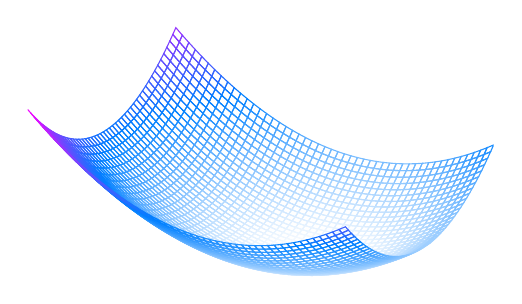
\begin{tikzpicture}
\begin{axis}[
    hide axis,
    colormap/cool,
]
\addplot3[mesh,samples=50,domain=-8:8]{(x-2)^2+(y-1)^2};
\end{axis}
\end{tikzpicture}
\end{center}

\end{frame}

% -----------------------------------------------------------------------------

\begin{frame}
\frametitle{Aspects of CV Problems}

CV is about
\begin{itemize}
    \item Infering information about the world
    \item From images or videos (or extracted features)
\end{itemize}

\bigskip
To make things more formal, we represent
\begin{itemize}
    \item This information as a scalar $w$ or vector $\vw$
    \item Our measurements as a \emph{feature vector} $\vx$
\end{itemize}

\bigskip
We then \emph{model} the relationship between $\vx$ and $\vw$
\begin{itemize}
    \item Usually the most challenging aspect
\end{itemize}

\end{frame}

% -----------------------------------------------------------------------------

\begin{frame}
\frametitle{Aspects of CV Problems}

So each CV problem consists of three things
\begin{itemize}
    \item The information $\vw$ we are interested in
    \item The \emph{features} $\vx$ from which we infer this information
    \item A \emph{model} that describes the relationship
\end{itemize}

\bigskip
This model 
\begin{itemize}
    \item Is a mathematical function
    \item That usually has parameters that are learned from data
\end{itemize}

\end{frame}

% -----------------------------------------------------------------------------

\begin{frame}
\frametitle{Approaching CV Problems}

Thus we can break down every CV problem into
\begin{enumerate}
    \item Specifying $\vw$
    \item Specifying how we obtain $\vx$ (image processing)
    \item Modeling the relationship between $\vx$ and $\vw$
    \item Learning the particular relationship from \emph{training samples}
    \item Assessing the performance on \emph{test samples}
\end{enumerate}

\bigskip
We will discuss these steps using two example applications

\end{frame}

% -----------------------------------------------------------------------------

\begin{frame}
\frametitle{Approaching CV Problems}
\framesubtitle{Application 1}

Detect motion in videos via background subtraction

\bigskip
\begin{center}
    \copyrightbox[b]
    {\includegraphics[width=9cm]{figures/bgsub.png}}
    {\centering Image from \cite{prince12}}
\end{center}

\end{frame}

% -----------------------------------------------------------------------------

\begin{frame}
\frametitle{Approaching CV Problems}
\framesubtitle{Application 1 -- Selecting $\vw$}

We want to predict whether a pixel belongs to a moving object

\bigskip
We are interested in a single property with two possible outcomes
\begin{itemize}
    \item A pixel either belongs to a moving object or not
    \item So $\dim(\vw)=1$ and we just write $w$
    \item We let $w=1$ mean yes and $w=0$ mean no
\end{itemize}

\bigskip
As $w\in\{0,1\}\subset\NN$, this is a \emph{classification problem}

\end{frame}

% -----------------------------------------------------------------------------

\begin{frame}
\frametitle{Approaching CV Problems}
\framesubtitle{Application 1 -- Selecting $\vx$}

Given our problem we
\begin{itemize}
    \item Build a model independently for each pixel % because different pixels obviously depict different objects
    \item Let $\vx=(r,g,b)$ be the corresponding pixel value
\end{itemize}

\bigskip
We decide that color should not matter and convert to grayscale
\begin{itemize}
    \item We end up with a single value $x\in\{0,\dots,255\}$ % assuming 8-bit images
\end{itemize}

\end{frame}

% -----------------------------------------------------------------------------

\begin{frame}
\frametitle{Approaching CV Problems}
\framesubtitle{Application 1 -- Model Selection}

Suppose that it is reasonable to assume that
\begin{itemize}
    \item The illumination remains constant % e.g. indoors, no windows
    \item The sensor noise is normally distributed % sensor noise often is
    \item We don't know how moving objects look like % because we don't know apriori what we will see
    \item Moving and unmoving objects are equally likely
\end{itemize}

\bigskip
We build a \emph{statistical model} $\Pr(x|w)$ % this is short for Pr(x=some_x|w=some_w)
\begin{itemize}
    \item Probability that a pixel assumes value $x$, given a certain $w$
\end{itemize}

\bigskip
As we model $x$ given $w$, this is a \emph{generative model}

\end{frame}

% -----------------------------------------------------------------------------

\begin{frame}
\frametitle{Approaching CV Problems}
\framesubtitle{Application 1 -- Model Selection}

Given these assumptions, we have % second, third, fourth list in previous itemize
\begin{eqnarray*}
    \Pr(x|w=0)&=&\Norm_{x}(\mu,\sigma^2)\\ % this means "normal distribution with mu, sigma^2 evaluated at x"
    \Pr(x|w=1)&=&\Uniform_x(0, 255) \\ % we assume we have 8bit information, so a brightness between 0 and 255, and that we don't know anything about the distribution of foreground objects
    \Pr(w)&=&\Bern_w(0.5) % Bernoulli distribtuion, Pr(w=0) = lambda, Pr(w=1) = 1-lambda
\end{eqnarray*}


\end{frame}

% -----------------------------------------------------------------------------

\begin{frame}
\frametitle{Approaching CV Problems}
\framesubtitle{Application 1 -- Learning}

We need to learn the \emph{model parameters} $\bth=(\mu,\sigma)$

\bigskip
So we collect $n$ frames in which no motion occurs
\begin{itemize}
    \item Let $\{x_i\}_{i=1}^n$ be the training set for a given pixel
\end{itemize}

\bigskip
We don't know anything about $\mu$ and $\sigma$ so we
\begin{itemize}
    \item Assume that the training samples are independent % we always assume this
    \item Estimate $\bth$ purely from data (\emph{maximum likelihood}) % we select mu and sigma so that the observed samples become maximally likely
\end{itemize}

\end{frame}


% -----------------------------------------------------------------------------

\begin{frame}
\frametitle{Approaching CV Problems}
\framesubtitle{Application 1 -- Learning}

Maximum likelihood means selecting the $\bth$
\begin{itemize}
    \item Under which observing $\{x_i\}_{i=1}^n$ is most likely
\end{itemize}

\bigskip
Or in mathematical terms
\begin{eqnarray*}
  \hat{\bth}&=&\argmax_{\bth}\,\Pr(x_1,\dots,x_n|\bth) \\ % this is maximum likelihood - we find the theta that maximizes the likelihood of our data  
  &=&\argmax_{\bth}\prod_{i=1}^n \Pr(x_i|\bth) % because samples are statistically independent (iid)
\end{eqnarray*}

\end{frame}

% -----------------------------------------------------------------------------

\begin{frame}
\frametitle{Approaching CV Problems}
\framesubtitle{Application 1 -- Learning}

Continuing from before 
\begin{eqnarray*}
  \hat{\bth}&=&\argmax_{\bth}\prod_{i=1}^n \Norm_{x_i}(\mu,\sigma^2) \\ % normal distribution because that's the model we have decided to use
  &=&\argmax_{\bth}\sum_{i=1}^n\log \Norm_{x_i}(\mu,\sigma^2) \\ % take the logarithm, which makes optimization easier (logarithm is monotonic so it wont change result)
  &=&\argmax_{\bth}\left(-0.5 n\log\sigma^2-0.5n\log(2\pi) - 0.5\sum_{i=1}^n\frac{(x_i-\mu)^2}{\sigma^2}\right)
\end{eqnarray*}

\end{frame}

% -----------------------------------------------------------------------------

\begin{frame}
\frametitle{Approaching CV Problems}
\framesubtitle{Application 1 -- Learning}

If we differentiate and equate to zero, we obtain % at the max the first derivate is 0. see Prince's book for details. you don't have to be able to derive these equations for the exam
\begin{eqnarray*}
    \hat{\mu}&=&\frac{1}{n}\sum_{i=1}^n x_i \\\medskip
    \hat{\sigma}^2&=&\frac{1}{n}\sum_{i=1}^n \left(x_i-\hat{\mu}\right)^2
\end{eqnarray*}

\bigskip
We have derived \emph{algorithms} for finding our model parameters

\end{frame}

% -----------------------------------------------------------------------------

\begin{frame}
\frametitle{Approaching CV Problems}
\framesubtitle{Application 1 -- Inference}

To obtain $w$ from $\Pr(x|w)$ we use \emph{Bayes' rule}
\[
    \Pr(w|x) = \frac{\Pr(x|w)\Pr(w)}{\Pr(x)}
\]

\bigskip
Or if we don't need probabilities, we simply assign $w=0$ iff
\[
    \Pr(x|w=0)\Pr(w=0) > \Pr(x|w=1)\Pr(w=1)
\]

\end{frame}

% -----------------------------------------------------------------------------

\begin{frame}
\frametitle{Approaching CV Problems}
\framesubtitle{Application 1 -- Inference}

Assume we learned $\mu=95,\sigma=2$ and observe $x=100$

\bigskip
We obtain
\begin{itemize}
    \item $\Pr(x=100|w=0)\Pr(w=0)=\text{Norm}(100;95,2)\cdot 0.5$
    \item $\Pr(x=100|w=1)\Pr(w=1)=\text{Uniform}(0,255)\cdot 0.5$
    \item We get $0.004$ and $0.002$, respectively, so $w=0$
\end{itemize}

\end{frame}

% -----------------------------------------------------------------------------

\begin{frame}
\frametitle{Approaching CV Problems}
\framesubtitle{Application 1 -- Inference}

For probabilities we divide by $\Pr(x=100)$ (Bayes rule) \\\medskip
We obtain $\Pr(x=100)$ via \emph{marginalization}

\bigskip
Recall from statistics lecture that
\begin{itemize}
    \item $\Pr(x)=\sum_w\Pr(x,w)$ (discrete case)
    \item $\Pr(x,w)=\Pr(x|w)\Pr(w)$
\end{itemize}

\bigskip
So $\Pr(x=100)=\sum_{i\in\{0,1\}}\Pr(x=100|w=i)\Pr(w=i)\approx.006$  % we already calculated this above
\begin{itemize}
    \item We already calculated the summands in previous slide
\end{itemize}

\end{frame}

% -----------------------------------------------------------------------------

\begin{frame}
\frametitle{Approaching CV Problems}
\framesubtitle{Application 1 -- Remarks}

Model selection governed by \emph{domain knowledge}
\begin{itemize}
    \item Illumination does not change
    \item Sensor noise is normally distributed
    \item No information on moving object frequency, appearance
\end{itemize}

\bigskip
If you have this information, \emph{this is the way to go}
\begin{itemize}
    \item Think about how your data came into being
    \item Use this information for modeling
\end{itemize}

\end{frame}

% -----------------------------------------------------------------------------

\begin{frame}
\frametitle{Approaching CV Problems}
\framesubtitle{Application 1 -- Remarks}

On this basis your solution \textit{will work} unless
\begin{itemize}
    \item The assumptions were wrong (e.g.\ illumination changes)
    \item Training data are not representative ($\hat{\bth}$ wrong)
\end{itemize}

\end{frame}

% -----------------------------------------------------------------------------

\begin{frame}
\frametitle{Approaching CV Problems}
\framesubtitle{Application 2}

Categorize naturalistic images into thousands of classes

\bigskip
\begin{center}
    \copyrightbox[b]
    {\includegraphics[width=9cm]{figures/imagenet.jpg}}
    {\centering Image from \url{image-net.org}}
\end{center}

\end{frame}

% -----------------------------------------------------------------------------

\begin{frame}
\frametitle{Approaching CV Problems}
\framesubtitle{Application 2 -- Selecting $\vw$}

Assume there is a single dominant object in each image \\\medskip
Goal is to predict which object is visible

\bigskip
Classification problem with $c$ classes, $w\in\{0,\dots,c-1\}$

\end{frame}

% -----------------------------------------------------------------------------

\begin{frame}
\frametitle{Approaching CV Problems}
\framesubtitle{Application 2 -- Selecting $\vx$}

What are good features for this task?
\begin{itemize}
    \item No clear relationship between images and $w$
    \item Thus unclear how to select $\vx$
\end{itemize}

\bigskip
So we just resize the images to a fixed size $u\times v$ \\\medskip
And use a powerful model that figures out the rest

\end{frame}

% -----------------------------------------------------------------------------

\begin{frame}
\frametitle{Approaching CV Problems}
\framesubtitle{Application 2 -- Model Selection}

We use a \emph{Convolutional Neural Network} (\emph{CNN})
\begin{itemize}
    \item Special kind of neural network (details later)
    \item Known to perform exceptionally well in such cases
\end{itemize}

\bigskip
CNNs are \emph{discriminative models}, $\Pr(w|\vx)$  % they are usually used as such, but they can also be used generatively. also cnns are not necessarily probabilistic (depends on the layer configuration), but usually they are
\begin{itemize}
    \item Compare to the generative model in application 1
\end{itemize}

\end{frame}

% -----------------------------------------------------------------------------

\begin{frame}
\frametitle{Approaching CV Problems}
\framesubtitle{Application 2 -- Model Selection}

CNNs consist of several layers we must specify manually
\begin{itemize}
    \item Such model parameters are called \emph{hyperparameters}
    \item More familiar example: $k$ in $k$-means
\end{itemize}

\bigskip
Typically specified
\begin{itemize}
    \item Based on experience, literature
    \item Experimentally (try and see what works best)
\end{itemize}

\end{frame}

% -----------------------------------------------------------------------------

\begin{frame}
\frametitle{Approaching CV Problems}
\framesubtitle{Application 2 -- Learning}

Assume that we again have $n$ training samples $\{(\vx_i,w_i)\}_{i=1}^n$
\begin{itemize}
    \item $w_i$ is class of visible object in image $\vx_i$
\end{itemize}

\bigskip
Proceeding as in application 1 we seek % iid samples, maximum likelihood
\begin{eqnarray*}
  \hat{\bth}&=&\argmax_{\bth}\,\Pr(w_1,\dots,w_n|\vx_1,\dots,\vx_n,\bth) \\\medskip
  &=&\argmax_{\bth}\prod_{i=1}^n \Pr(w_i|\vx_i,\bth) \\\medskip
  &=&\argmax_{\bth}\sum_{i=1}^n \log\Pr(w_i|\vx_i,\bth)
\end{eqnarray*}

\end{frame}

% -----------------------------------------------------------------------------

\begin{frame}
\frametitle{Approaching CV Problems}
\framesubtitle{Application 2 -- Learning}

But our model $\Pr(w|\vx,\bth)$ is very complex
\begin{itemize}
    \item CNNs can have millions of parameters
    \item Computing $\Pr(w|\vx,\bth)$ can require millions of operations
    \item There is no analytical solution
\end{itemize}

\bigskip
Thankfully algorithms for learning already exist

\end{frame}

% -----------------------------------------------------------------------------

\begin{frame}
\frametitle{Approaching CV Problems}
\framesubtitle{Application 2 -- Inference}

Our model is discriminative so we don't need Bayes' rule
\begin{itemize}
    \item We have modeled $\Pr(w|\vx)$ directly
\end{itemize}

\end{frame}

% -----------------------------------------------------------------------------

\begin{frame}
\frametitle{Approaching CV Problems}
\framesubtitle{Application 2 -- Remarks}

No obvious relationship between images and $w$
\begin{itemize}
    \item Unclear how to select $\vx$
    \item Unable to model the relationship like before
\end{itemize}

\bigskip
For these reasons we
\begin{itemize}
    \item Use a powerful generic machine learning technique as model
    \item Incorporate feature selection into it
\end{itemize}

\end{frame}

% -----------------------------------------------------------------------------

\begin{frame}
\frametitle{Approaching CV Problems}
\framesubtitle{Application 2 -- Remarks}

CNNs are state of the art models for many CV problems
\begin{itemize}
    \item But very complex, require lots of training data
    \item More on CNNs later
\end{itemize}

\end{frame}

% -----------------------------------------------------------------------------

\begin{frame}
\frametitle{Approaching CV Problems}

Both applications were extreme (but realistic) examples

\bigskip
Application 1
\begin{itemize}
    \item Selecting and computing $\vx$ was trivial
    \item Derived statistical model and algorithms % for learning, inference
\end{itemize}

\bigskip
Application 2
\begin{itemize}
    \item Unclear how to select $\vx$
    \item Used a powerful model that did all the work
\end{itemize}

\end{frame}

% -----------------------------------------------------------------------------

\begin{frame}
\frametitle{Approaching CV Problems}

Most CV problems lie somewhere in between
\begin{itemize}
    \item Focus on obtaining suitable $\vx$ (image processing)
    \item Utilize generic machine learning algorithms as models
\end{itemize}

\bigskip
We will see a few examples in upcoming lectures

\end{frame}

% -----------------------------------------------------------------------------

\begin{frame}
\frametitle{Approaching CV Problems}
\framesubtitle{Suggestions}

Think about how your data came into being \\\medskip
Use this information to model the relationship between $\vx$ and $\vw$ \\\medskip
Ideally use probabilistic models (model uncertainty)

\end{frame}

% -----------------------------------------------------------------------------

\begin{frame}
\frametitle{Approaching CV Problems}
\framesubtitle{Suggestions -- Models vs.\ Algorithms}

Don't think in terms of algorithms

\bigskip
\enquote{I will use a linear SVM to predict the class}
\begin{itemize}
    \item Is this even a suitable model for the given problem?
\end{itemize}

\bigskip
Go the other way around
\begin{itemize}
    \item Confirm that a linear \textit{model} is applicable
    \item Select a suitable \textit{algorithm} (e.g.\ linear SVM)
\end{itemize}

\end{frame}

% -----------------------------------------------------------------------------

\begin{frame}
\frametitle{Approaching CV Problems}
\framesubtitle{Suggestions}

Embrace machine learning
\begin{itemize}
    \item It is everywhere in modern CV (including image processing)
    \item Don't guess your parameters, learn them
\end{itemize}

\end{frame}

% -----------------------------------------------------------------------------

\begin{frame}
\frametitle{Approaching CV Problems}
\framesubtitle{Suggestions}

Don't reinvent the wheel
\begin{itemize}
    \item Others likely have worked on similar problems
\end{itemize}

\bigskip
Use online libraries
\begin{itemize}
    \item IEEE (\href{http://ieeexplore.ieee.org/}{\texttt{ieeexplore.ieee.org}}), ACM (\href{http://dl.acm.org/}{\texttt{dl.acm.org}}), Google Scholar
\end{itemize}

\bigskip
Use (good) libraries instead of starting from scratch
\begin{itemize}
    \item We have already seen a selection
\end{itemize}

\end{frame}

% -----------------------------------------------------------------------------

\renewcommand\emph[1]{\oldemph{#1}}

\begin{frame}
\frametitle{Bibliography}

\printbibliography

\end{frame}

\end{document}
